\chapter{ATLAS}
\label{chap:ATLAS}

In this Chapter the ATLAS Pixel detector will be discussed, with a special focus on radiation
 damage. 
After a short introduction to the Large Hadron Collider (LHC) Physics program in 
Section~\ref{sec:LHCPhysics}, the ATLAS detector, one of the experiments at the LHC, will be 
presented (Section~\ref{sec:ATLASDetector}). Particular emphasis will be devoted to the 
the ATLAS Pixel Detector (Section~\ref{sec:ATLASPixelDetector}), before moving to the 
core of this Chapter - Section~\ref{sec:digitizer} -
 where the modelization of the radiation damage to the ATLAS Pixel 
Detector will be discussed. Finally, the impact of Radiation Damage on Higgs Analysis 
will be presented in Section~\ref{sec:raddamHiggs}; this is a study case that is in 
perspective very important given the excellent luminosity performance of LHC as we write.

\section{The LHC Physics Program}
\label{sec:LHCPhysics}
Understanding the nature of electroweak symmetry breaking, and in particular  specifically 
deciphering the Higgs mechanism, is the main goal of the ATLAS~\cite{AtlasDetector} and 
CMS~\cite{CMSDetector} experiments at the LHC~\cite{LHCMachine}. 

The LHC is an hadron accelerator and collider located about 100~m underground, in the former 
Large Electron Positron (LEP) collider tunnel, at the French-Swiss border in the vicinity of Geneva. As LEP, LHC too was built by CERN, the European 
Organization for Nuclear Research. The LHC has a circumference of 27~km and uses 
superconducting magnets to bend proton beams with energy up to a design value of 7~TeV; hence 
the maximum achievable center-of-mass energy $\sqrt{s}$ for $pp$ collisions is of 14~TeV. The design instantaneous 
luminosity of the LHC is of $L=1.0\times10^{34}$/cm$^{2}$/s, which is equivalent to 10/nb/s. 
The $pp$ total cross section $\sigma_{tot}$ at $\sqrt{s}$ of 14~TeV is about 10$^8$~nb, 
so the event rate at LHC is in the order of 10$^9$~Hz. 
The protons are packed in bunches of about 10$^{11}$ particles; the bunch crossing frequency $\nu$ is 
of 40~MHz.  The ratio of event rate to $\nu$ gives the average number of $pp$ collisions per 
bunch crossing, the so-called {\it pile-up}; it is customary indicated with $\mu$ and for the LHC 
design values is of about 25 interactions per bunch crossing.

At the LHC the physics cross-sections are dominated by QCD 
jet production, which
is many orders of magnitude larger than the production of the
most interesting physics
channels. The latter are usually characterised by electroweak cross-sections. Figure~\ref{fig:sec1_cross_lhc} shows the production cross-sections for several
representative processes at hadron colliders, as a function of the center-of-mass energy.
It can be seen that the  production cross section of a light Higgs is of the order of several tens of nb so 
the Higgs boson is produced about once every billion collisions of the LHC.

\begin{figure}[!htbp]
\centering
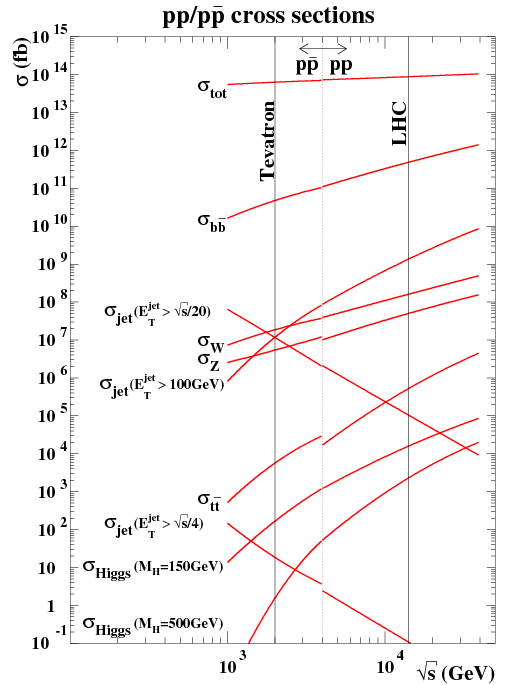
\includegraphics[width=0.43\textwidth]{sec1_cross_lhc.png}
\caption{\label{fig:sec1_cross_lhc}Production cross-sections for several represe
ntative processes at hadron colliders. (After~\cite{Weiglein:2004hn})}
\end{figure}

As already mentioned in Chapter~\ref{chap:context}
the two collaborations have both observed a boson compatible with the SM Higgs in 2012; 
since then the nature of that particle and its coupling to fundamental SM bosons and fermions 
keep being pursued.  Recently ATLAS reported evidence of $H\to\b\b$ decay~\cite{ATLASHbb2017} 
when produced in association with a $W$ or $Z$ boson; the CMS collaboration announced 
the first observation of Higgs boson decays to $\tau$ leptons~\cite{CMSHtautau2017}. 
The search for the Higgs boson decaying to second generation fermions is next on the 
agenda of the ATLAS and CMS collaborations (example:~\cite{ATLASHmumu2017}).

Other than the Higgs, a central goal of the physics program of the LHC is the exploration of particles and 
interactions at the TeV energy scale, which may hold answers to some of the most profound questions in 
particle physics, like what is dark matter made of and how the Higgs boson mass gets stabilised.

The total delivered luminosity so far from the LHC to the ATLAS experiment  is shown in 
Figure~\ref{fig:intlumivsyear}~\cite{ATLASLumi}.

\begin{figure}[!htpb]
\centering
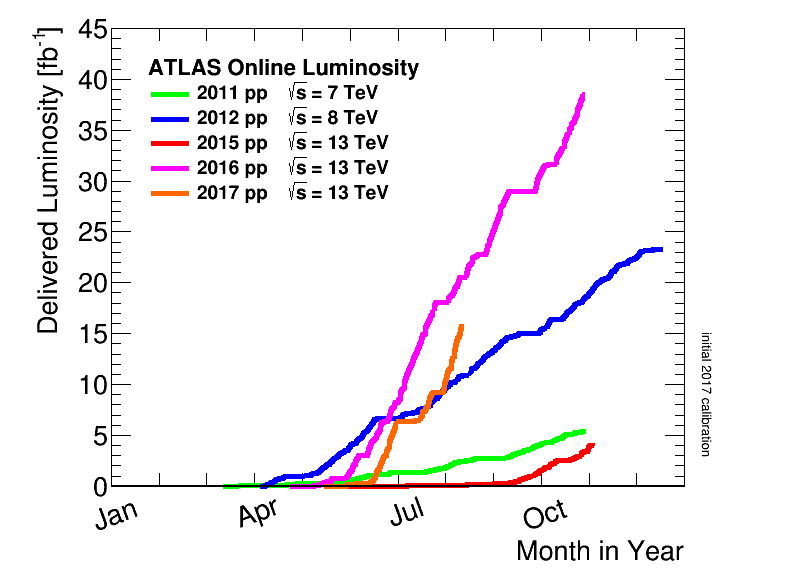
\includegraphics[width=0.62\textwidth]{intlumivsyear.png}
\caption{\label{fig:intlumivsyear}Cumulative luminosity versus day delivered to ATLAS during stable 
beams and for high energy p-p collisions. (After~\cite{ATLASLumi})}
\end{figure}

To exploit at best this dataset, to perform precision measurements 
and to face the high interaction rates, radiation doses, particle multiplicities and energies of 
LHC $pp$ collisions the ATLAS detector was built. In the next Section the salient features of this 
detector will be presented.

\section{The ATLAS Detector}
\label{sec:ATLASDetector}
ATLAS~\cite{AtlasDetector} is a general-purpose particle detector covering nearly the entire solid 
angle\footnote{ATLAS uses a right-handed coordinate system with its origin at the nominal interaction 
point (IP) in the centre of the detector and the $z$-axis coinciding with the axis of the beam pipe.  The 
$x$-axis points from the IP towards the centre of the LHC ring, and the $y$-axis points upward. 
Cylindrical coordinates ($r$,$\phi$) are used in the transverse plane, $\phi$ being the azimuthal angle 
around the $z$-axis. The pseudorapidity is defined in terms of the polar angle $\theta$ as $\eta = - \ln 
\tan(\theta/2)$. The distance in ($\eta$,$\phi$) coordinates, $\Delta R = \sqrt{(\Delta\phi)^2+
(\Delta\eta)^2}$, is also used to define cone sizes. Transverse momentum and energy are defined as $
\pt=p\sin\theta$ and $\et=E\sin\theta$, respectively.} around the collision point. It consists of an inner 
tracking detector surrounded by a thin superconducting solenoid, electromagnetic and hadronic 
calorimeters,
and a muon spectrometer incorporating three large superconducting toroidal magnets. 
Figure~\ref{fig:ATLASDetector} shows a schematic view of the ATLAS detector.

\begin{figure}[!htpb]
\centering
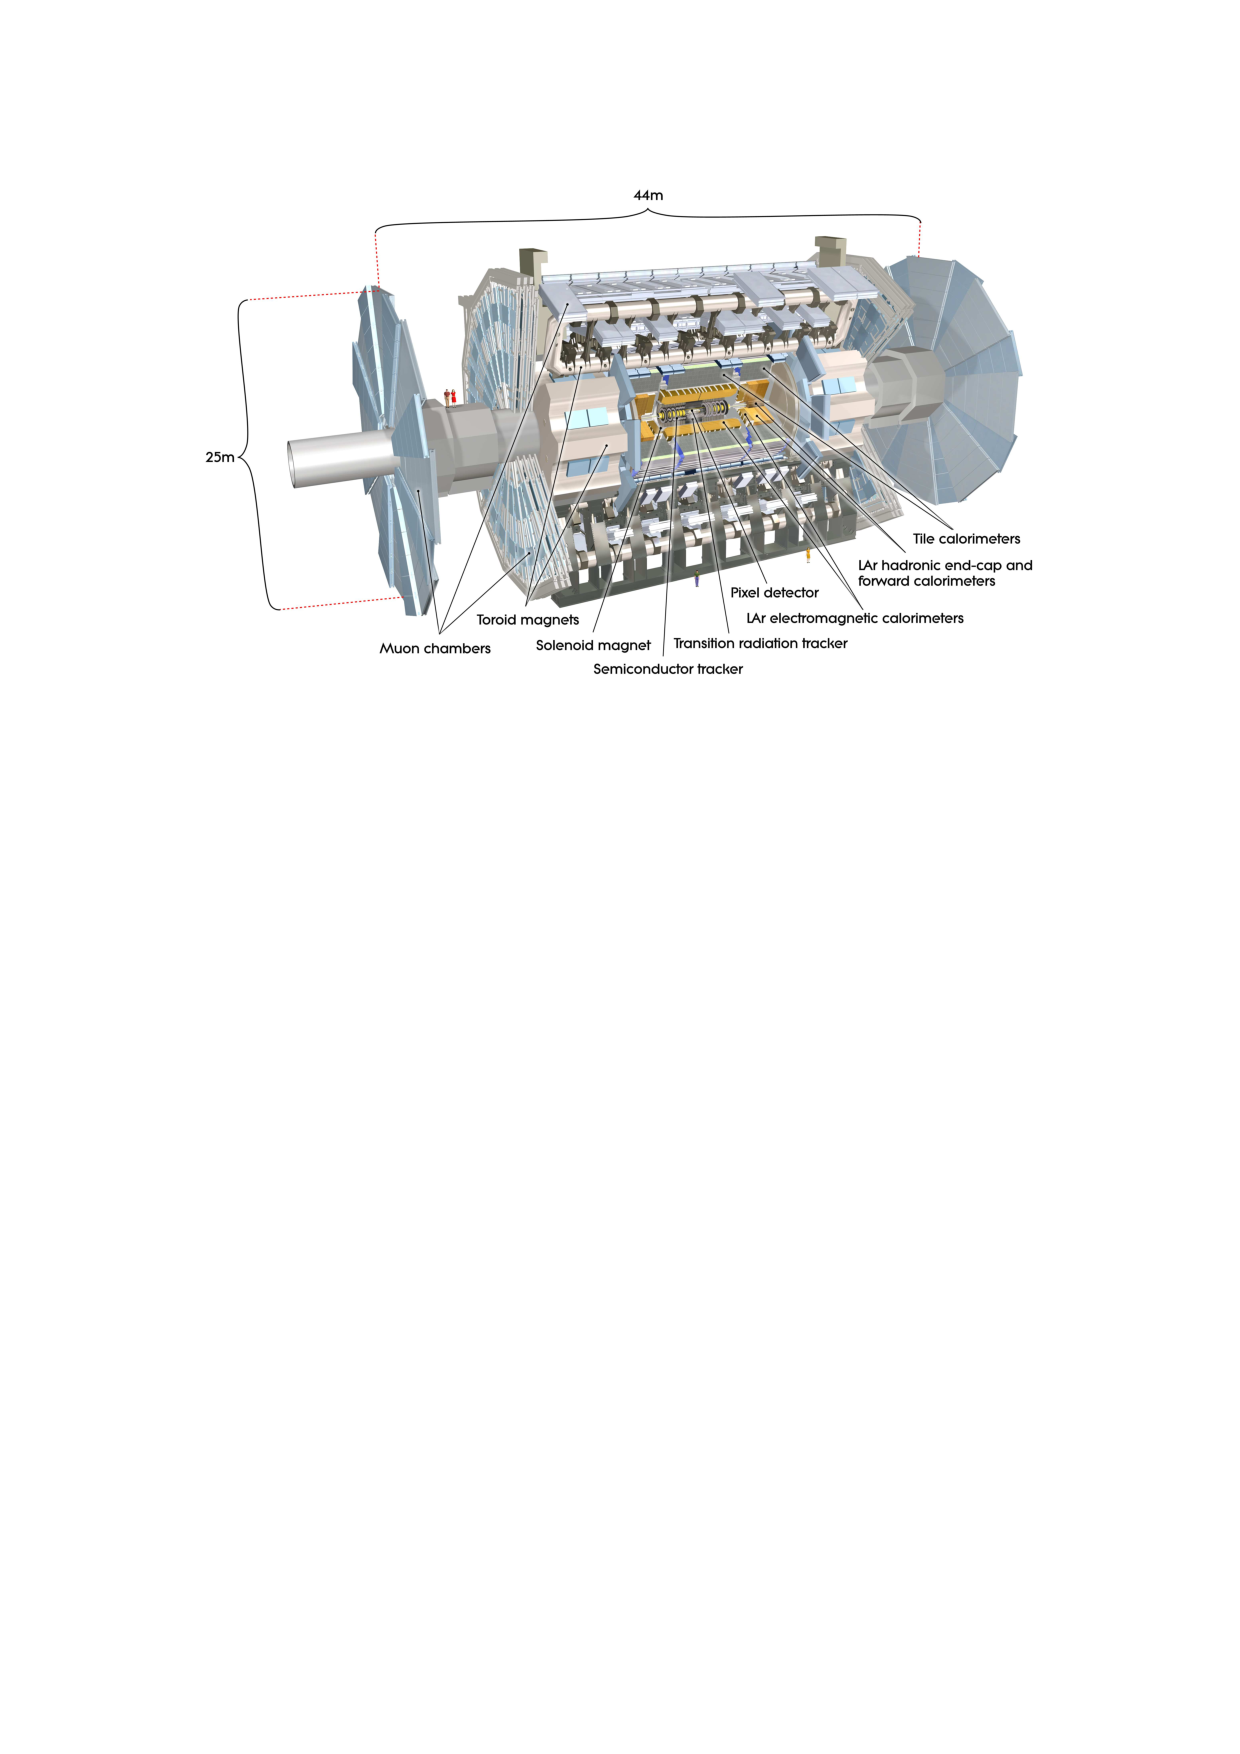
\includegraphics[width=0.65\textwidth]{ATLASDetector.pdf}
\caption{\label{fig:ATLASDetector}Cut-away view of the ATLAS detector. The dimensions of the detector are 25 m in height and 44 m in length. The overall weight of the detector is approximately 7000 tonnes.
 (After~\cite{AtlasDetector})}
\end{figure}


The inner tracking detector (ID or {\it inner detector}), located within a 2~T axial magnetic field generated by the superconducting solenoid, is used to measure the trajectories and momenta of charged particles. The inner layers, consisting of high-granularity silicon pixel detectors, instrument a pseudorapidity
range $|\eta| < 2.5$.
A new innermost silicon pixel layer, the insertable B-layer~\cite{IBLTDR} (IBL), was added to the detector between the first two LHC runs (Run~1 and Run~2). The IBL improves the ability to identify displaced vertices and thereby significantly improves the $b$-tagging performance~\cite{ATL-PHYS-PUB-2015-022}. More details 
on the pixel detector will be given in the next Section.
Silicon strip detectors covering $|\eta| < 2.5$ are located beyond the pixel detectors. 
Outside the strip detectors and covering $|\eta | < 2.0$, there are straw-tube tracking detectors, which also provide measurements of transition radiation that are used in electron identification.
Figure~\ref{fig:ATLASID} shows the barrel section of the ID.

\begin{figure}[!htbp]
\centering
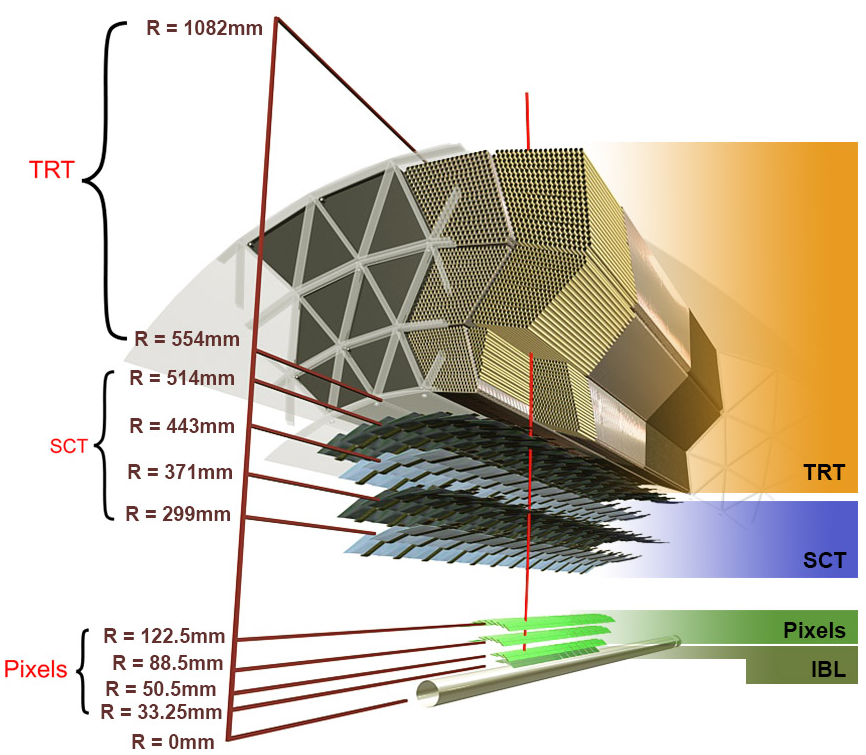
\includegraphics[width=0.65\textwidth]{ATLAS_ID.png}
\caption{\label{fig:ATLASID}Schematic view of the  barrel part of the ATLAS Inner Detector (ID), including the new Insertable B-Layer (IBL). (After~\cite{Potamianos:2016ptf})}
\end{figure}


The calorimeter system covers the pseudorapidity range $|\eta| < 4.9$.
Within the region $|\eta|< 3.2$, electromagnetic calorimetry is provided by barrel ($|\eta| < 1.475$) and
endcap ($1.375 < |\eta| < 3.2$) high-granularity lead/liquid-argon (LAr) electromagnetic calorimeters,
with an additional thin LAr presampler covering $|\eta| < 1.8$ to correct for energy loss in material upstream of the calorimeters.
Hadronic calorimetry is provided by a steel/scintillator-tile calorimeter, segmented into three barrel structures within $|\eta| < 1.7$, and two copper/LAr hadronic endcap calorimeters extend the coverage to $|\eta|=3.2$.
The solid angle coverage for $|\eta|$ between 3.2 and 4.9 is completed with copper/LAr and tungsten/LAr calorimeter modules optimised for electromagnetic and hadronic measurements, respectively.

The outermost part of the detector is the muon spectrometer, which measures the curved trajectories of muons in the field of three large air-core toroidal magnets. High-precision tracking is performed within the range $|\eta| < 2.7$ and there are chambers for fast triggering within the range $|\eta| < 2.4$.

The proton-proton interaction rate at the design luminosity of $L=1.0\times10^{34}$/cm$^{2}$/s 
is approximately 1 GHz, while the event data recording, based on technology and resource limitations, 
is limited to about 200 Hz. For this purpose ATLAS designed 
a three-level trigger system selects events to be recorded for offline analysis, to assure 
an overall rejection factor of $5\times10^{6}$ against minimum-bias processes while maintaining 
maximum efficiency for the new physics. 
The Level-1 (L1) trigger system uses a subset of the total detector information to make a decision on 
whether or not to continue processing an event, reducing the data rate to approximately 75~kHz (limited 
by the bandwidth of the readout system, which was upgraded to 100~kHz between Run~1 and Run~2). 
The subsequent two levels, 
collectively known as the high-level trigger, are the Level-2 (L2) trigger and the event filter. They provide 
the reduction to a final data-taking rate of approximately 200~Hz (upgraded to 100~kHz between 
Run~1 and Run~2)~\cite{AtlasTrigger2015}. A new Fast TracKer (FTK) system~\cite{FTKTDR} will 
provide global ID track reconstruction at the L1 trigger rate
using lookup tables stored in custom associative memory chips for the pattern recognition.  This 
system is currently being installed and expected to
be fully commissioned by the end of 2017.


\section{The ATLAS Pixel Detector}
\label{sec:ATLASPixelDetector}


\begin{figure}[!htbp]
\centering
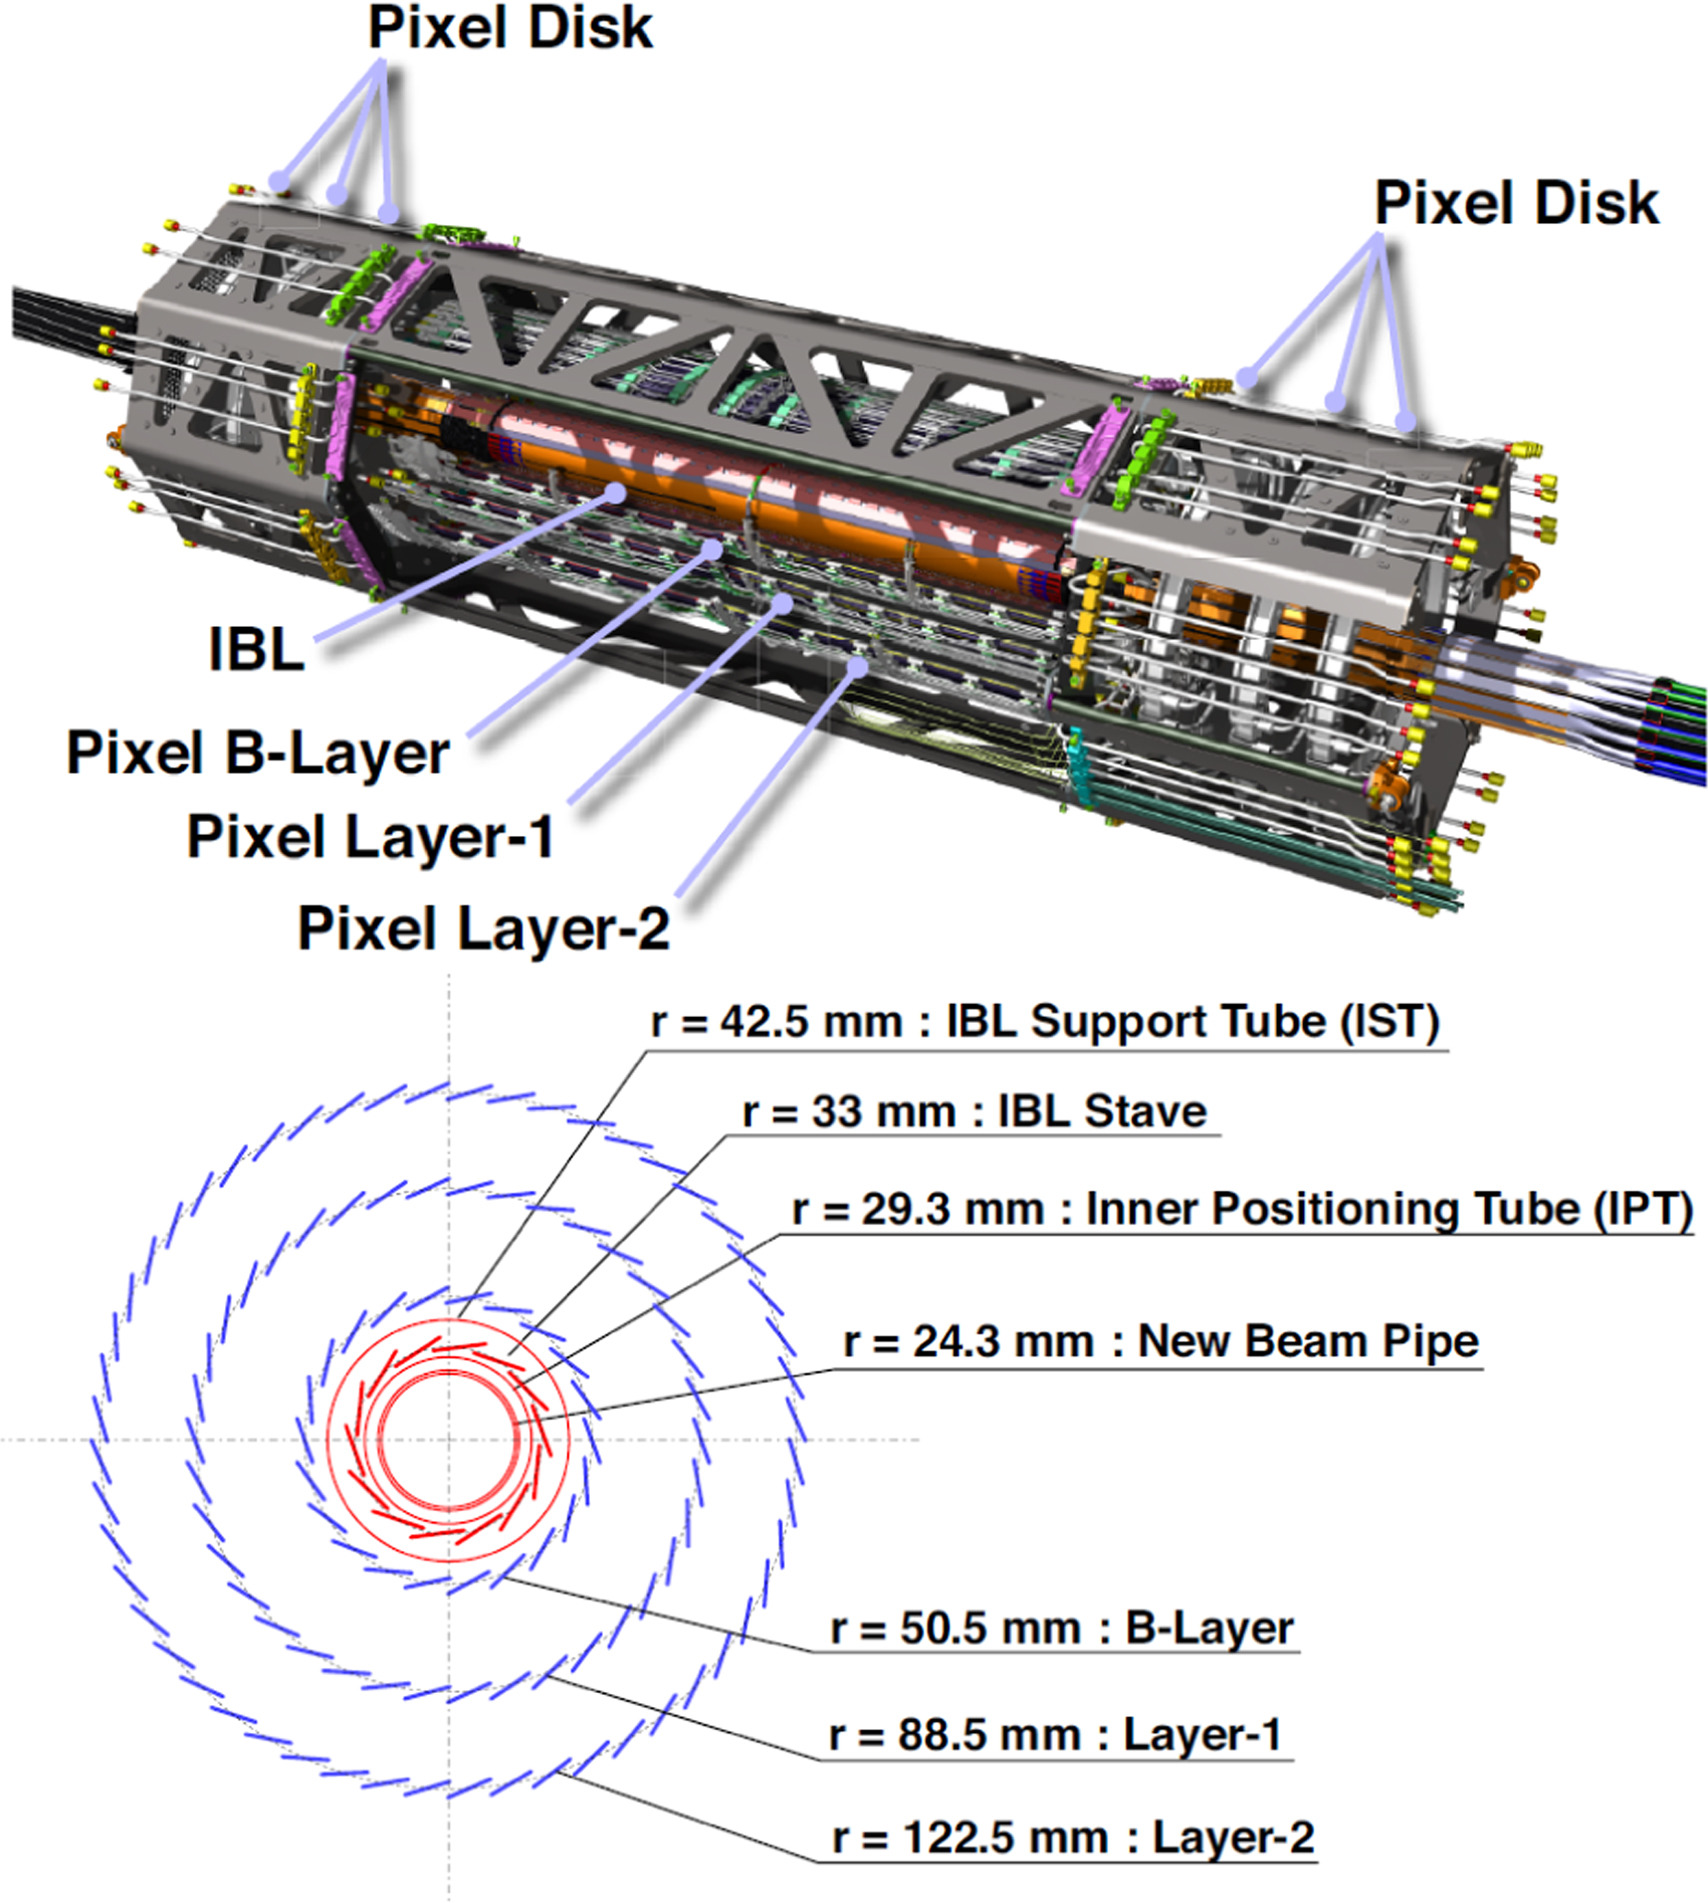
\includegraphics[width=0.65\textwidth]{ATLASPixels.jpg}
\caption{\label{fig:ATLASPixels}Schematic view of the ATLAS 4-Layer Pixel Detector for Run 2. (After~\cite{BACKHAUS201665})}
\end{figure}

\section{Radiation Damage to the ATLAS Pixel Detector}
\label{sec:digitizer}

\section{Impact of Radiation Damage on Higgs Analysis}
\label{sec:raddamHiggs}